\chapter{Metodologia}

A presente pesquisa adota uma abordagem de caráter exploratório, em virtude da ampla variedade de possibilidades de modelagem e implementação relacionadas ao problema de localização de facilidades. O processo de desenvolvimento seguirá a estratégia \textit{bottom-up}, iniciando-se pela construção de uma versão mínima da aplicação, em seu estado mais elementar, e avançando gradualmente por meio de incrementos sucessivos no escopo do projeto. Tal estratégia busca garantir uma evolução controlada, permitindo a ampliação das funcionalidades de forma contínua e sistemática. Para viabilizar esse processo, foi previamente estabelecida uma base estrutural sólida, que assegura a estabilidade do sistema e reduz a necessidade de alterações profundas no código durante a inserção de novos módulos e serviços. 

O andamento do projeto será orientado por metas semanais e pela dedicação contínua ao desenvolvimento. Devido à diversidade de componentes do projeto e à abordagem exploratória adotada, é esperado que surjam dificuldades ao longo do caminho, podendo ser necessário desconsiderar ou remover certas funcionalidades e, eventualmente, ajustar o fluxo de trabalho. Por essa razão, a elaboração de um cronograma rígido se torna praticamente inviável devido a natureza líquida da abordagem, já que mesmo que seja estabelecido, seu seguimento estrito pode não ser possível.

Diante disso, torna-se preferível estabelecer uma ordem de prioridade na implementação das funcionalidades, conforme descrito a seguir:
\begin{itemize}
    \item Interface: A interface do programa é considerada a camada mais importante, sendo, portanto, a primeira a ser desenvolvida. O foco inicial está na criação de grafos de forma interativa, com atenção à escalabilidade e usabilidade. Ao longo do projeto, as demais funcionalidades serão integradas à interface, garantindo uma evolução contínua.
    \item Representação: Após a definição de uma interface funcional, a próxima etapa é consolidar a representação interna dos dados no back-end, com atenção à eficiência e modularidade. Isso inclui decisões sobre a melhor forma de estruturar grafos (por exemplo, listas ligadas ou matrizes), definição de interfaces e contratos, e organização hierárquica das entidades no contexto do FLP. Embora esta etapa seja relativamente rápida, ajustes podem ser necessários à medida que novas funcionalidades forem implementadas ou otimizações de código forem identificadas.
    \item Algoritmos: Com a interface e a representação interna bem estabelecidas, inicia-se a implementação dos algoritmos que estarão disponíveis para o usuário, permitindo a realização de comparações e experimentos no ambiente.
\end{itemize}

A ideia central é adotar um modelo próximo ao \textit{waterfall}, em que cada etapa deve estar suficientemente definida antes da seguinte ser iniciada. Entretanto, não é necessário que uma fase esteja completamente concluída para avançar, já que uma base sólida garante a continuidade do desenvolvimento, permitindo progressos de forma controlada e iterativa. A Figura \ref{ciclo_dev} ilustra o processo em ciclos, onde o avanço para o próximo ciclo necessita de estabelecimento de uma base sólida no anterior

\begin{figure}[htb]
	\caption{\label{ciclo_dev}Ciclo de desenvolvimento}
	\begin{center}
	    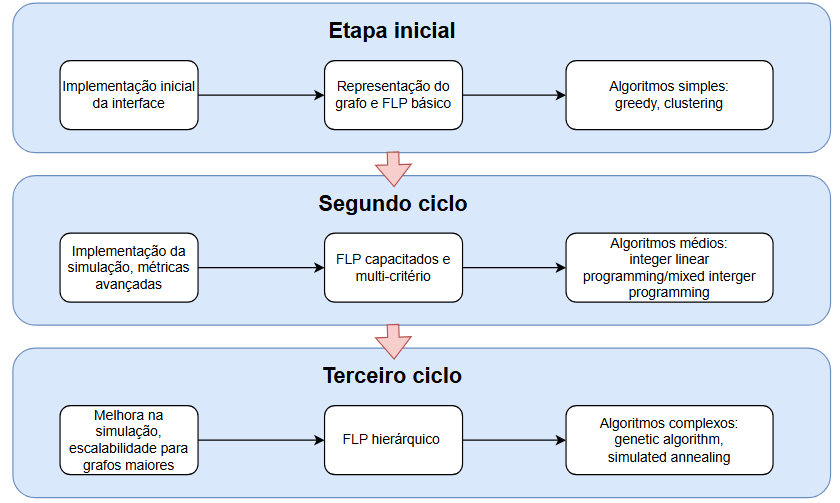
\includegraphics[scale=0.8]{imagens/ciclo_dev.png}
	\end{center}
	\legend{Fonte: Elaboração própria.}
\end{figure}

\FloatBarrier

É importante ressaltar que o ambiente de experimentação desenvolvido não possui caráter educacional. Seu objetivo não é o de ensinar conceitos relacionados a FLP e algoritmos correlatos, mas sim disponibilizar a pesquisadores, profissionais, estudantes e usuários familiarizados com o tema uma ferramenta prática para simulação. A aplicação contará com recursos para ajudar o processo de experimentação, acompanhado por um guia de utilização que orientará o usuário quanto às funcionalidades do programa e ao seu correto manuseio.

Assim como ocorre em problemas de otimização combinatória, a adoção de abordagens exploratórias nem sempre garante a obtenção da solução ótima. O desenvolvimento deste projeto por meio de múltiplas experimentações pode acarretar riscos e desafios, como tempo de execução elevado, dificuldades de escalonamento e eventuais problemas arquiteturais. Entretanto, é importante destacar que a aplicação não tem como objetivo inovar ou resolver todos os problemas do domínio, funcionando apenas como um ambiente de implementação de técnicas já conhecidas. Limitações inerentes a essas técnicas estarão refletidas na aplicação, sendo responsabilidade do usuário compreender essas restrições. Caso algum método se mostre inviável, sua substituição é facilitada pela ampla disponibilidade de alternativas e recursos na literatura, permitindo a adaptação e continuidade do estudo de forma flexível e controlada. 


\section{Aplicação}

\subsection{Modelagem do problema}
Esta seção visa descrever como os dados, como por exemplo o grafo, e os problemas estão estruturados no algoritmo. Poderão ser utilizados trechos de códigos ou diagramas UML para facilitar a visualização da representação.


\subsection{Algoritmos e critérios utilizados}
É fundamental destacar que, em virtude do caráter genérico da aplicação proposta, torna-se necessário avaliar diferentes critérios e algoritmos de forma conjunta, de modo a identificar aqueles que apresentam maior adequação ao domínio em questão. A utilização de certas técnicas depende das propriedades estruturais e matemáticas do problema tratado. Por exemplo, um algoritmo baseado em agrupamento contínuo não pode ser aplicado diretamente sobre um grafo cuja natureza é intrinsecamente discreta. Sendo assim, os algoritmos e critérios utilizados serão definidos e implementados ao longo do tempo de desenvolvimento do projeto

Ao longo do desenvolvimento do projeto, esta seção será utilizada para descrever os algoritmos e critérios disponíveis na aplicação. 

\subsection{Fluxo de Execução}
O usuário final irá entrar no site a partir de um navegador, na qual terá a opção de importar um grafo a partir de um arquivo ou criar um grafo do zero a partir das ferramentas interativas disponíveis. O usuário poderá criar nós e conectar estes usando arestas, e caso clique em um nó, uma janela mostrando suas propriedades será exibida e nela o usuário poderá editar configurações sobre o nó, como marcar ele como um produtor ou consumidor, definir o peso da conexão com outras arestas, definir algumas propriedades relacionadas ao FLP como custo de implementação, entre outras. Tendo seu grafo pronto, o usuário poderá iniciar uma simulação, na qual será responsável por estruturar como será o problema de localização, isto é definir os critérios e o algoritmo a serem utilizados. Ao terminar a simulação, será exibido os resultados obtidos para o usuário, dando a possibilidade de ele salvar estas informações. É importante lembrar que como um dos focos é comparação e otimização, o usuário pode definir diversas estruturas para o problema, selecionando conjuntos de critérios diferentes ou algoritmos diferentes para gerar todos os resultados de uma única vez.

Esta seção será posteriormente populada com várias imagens demonstrando um fluxo de uso padrão da aplicação, detalhando mais como os processos descritos acimas ocorrem de fato.

\section{Arquitetura}

\subsection{Servidor}
O back-end do programa será implementado utilizando o \textit{Spring Framework}, um conjunto de ferramentas para desenvolvimento de aplicações Java que facilita a criação de sistemas robustos e escaláveis, com ênfase nos módulos \textit{Spring Boot}, que permite configurações e inicialização rápida da aplicação, garantindo deploy eficiente, e \textit{Spring Web}, que fornece suporte ao gerenciamento de requisições HTTP, garantindo comunicação eficiente entre o servidor e a interface do usuário. Essa escolha permite a construção de um back-end escalável, modular e de fácil manutenção, adequado à natureza genérica e experimental do ambiente proposto, sendo que a ampla utilização do Spring em projetos e sua performance superior em comparação com outros \textit{frameworks} e bibliotecas que realizam funções similares reforçam sua adequação \cite{springboot-why}.

A linguagem utilizada, como mencionado anteriormente, será Java, cuja natureza orientada a objetos facilita a modelagem de relações hierárquicas, a definição de contratos entre estruturas e a reutilização de código por meio de herança e polimorfismo.

\subsection{Cliente}
A interface do programa será implementada utilizando o \textit{framework React.js}, que se destaca por permitir o desenvolvimento de aplicações \textit{Single Page Application} (SPA) de forma modular, por meio da reutilização de componentes. Essa abordagem torna o código mais organizado, facilita a manutenção e possibilita a criação de interfaces interativas e responsivas. O React também oferece atualização eficiente do DOM por meio do Virtual DOM, garantindo desempenho elevado mesmo em aplicações com grande quantidade de elementos gráficos. 

Uma das principais vantagens do React, é a utilização de uma linguagem \textit{JavaScript XML} (JSX) que  é uma extensão da linguagem JavaScript que permite escrever sintaxe parecida com HTML dentro do código, de forma a escrever componentes de forma facilitada. Para aproveitar os benefícios da tipagem forte, será usada a variante \textit{TypeScript XML} (TSX). Como o navegador padrão não consegue interpretar estas linguagens, é necessário passar por um processo de compilação convertendo estas linguagens para JavaScript puro. Para isso será utilizado o \textit{build tool Vite} que automatiza e otimiza todo o processo, incluindo a transformação de TSX em JavaScript, gerenciamento de módulos e atualização instantânea da interface durante o desenvolvimento.

A renderização dos grafos será realizada utilizando componentes \textit{Scalable Vector Graphics} (SVG), que criam elementos diretamente no DOM do navegador, facilitando a interação e a manipulação individual dos objetos. Diferentemente da renderização baseada em \textit{canvas}, que utiliza uma abordagem de \textit{bitmap}, uma matriz de pixels coloridos, o SVG mantém o conhecimento do navegador sobre cada componente, permitindo atualizações e interações mais simples. Embora a renderização em \textit{canvas} possa ser mais rápida, já que não precisa atualizar o DOM, ela exige que o desenvolvedor implemente grande parte da lógica de interação manualmente, o que aumenta a complexidade do código. Em sistemas com grande número de elementos gráficos, técnicas de renderização baseadas em \textit{bitmap}, como \textit{WebGL}, que aproveita a GPU para cálculos, tendem a apresentar melhor desempenho. Uma abordagem híbrida, que combina diferentes técnicas de renderização de acordo com o nível de zoom ou complexidade dos dados, é ideal em cenários onde o volume de informações pode variar entre simples e complexo.

\subsection{Serviços}
Conforme o desenvolvimento do programa, é possível a necessidade de implementar serviços para lidar com algoritmos complexos ou até mesmo garantir modularização de algum componente da aplicação. Um exemplo de serviço possível é uma API em linguagem Python que recebe dados do Servidor e utiliza-os 
para análises estatísticas ou computação de algum algoritmo. Os serviços implementados serão descritos nessa seção, dando ênfase no tipo de entrada e saída, bem como processamento interno.